\section{Contributions}
\\
In this section, we will provide an overview over the data set, the training structure, the network architecture, the hyperparameters and the used evaluation techniques. We will also briefly describe our prototype.  

    \subsection{Dataset}

    Currently, the dataset consists of 329 colored pictures with a mean size of 828X1244 which is pretty big compared to the resized training data. This particulary large gap is one of the problems that arose while training. The pictures are self-collected, mainly by browsing the web. Subjectively, the results from the search engine duckduckgo.com were superior to the one suggested by google.com or startpage.com since it offered are more accurate results when searching for key phrases in this specific context. \newline
    The most pictures were found when seeking for burning houses in California. Since the wildfires in California are caused by the effects of climate change, the relation is sound. \newline
    Additionally, a big chunk of pictures came from the recent bushfires in Australia. The rest of the images do not have a connection to a specific event. Most houses are wooden and are surrounded by trees and dry areas. Similar to Schmidt et al.\cite{schmidt2019visualizing}, we tried to avoid images with extraneous features to prevent many-to-many mappings. Also the brightness of the pictures is also quite intense on average what is caused by the blaze and which makes the fire the dominant feature. For retrieving the data from the storage directory and for the different kinds of data augmentation we used the PIL library. It offers a broad range of tools from which we used flipping, cropping, rotating and sharpening. Except for the singular flipping, each augmentation method was applied at least twice with varying parameters. Eventually, we ended up with around 3619 pictures usable for the training of the model.\\
    Beforehand, we resized the pictures to 300X300 pixel which were then later adjusted as well for the sake of comparing the outcome. The sizes we tried have a range from 50 to 250 pixels.\\
    The optimal size lays between 100 and 200 pixels because within that range it is possible to find features on the generated pictures without having to deal with matrix multiplications of enormous size.
    For a small fraction of tasks, as the conversion of the numpy array back to the image, we used functions provided by the Keras API for image processing.
    
    \subsection{Training Structure}
    Concerning the implementation of the network, we first looked at the code written by Ivan Vasilev, proposed in his book "Python Deep Learning" \cite{PythonDeepLearning} in the Chapter about Generative Models. Hereby, we followed his training procedure, however the rest was adjusted according to our project's needs. Because our dataset cannot be imported with being ready for use, an infrastructure for loading as well as for the conversion to multi-dimensional tensors became necessary.\\
    Additionally, the loading of previously saved models and the saving of pictures and of the Generator itself can be customized. Lastly, we included the possibility to evaluate the model performance via Inception Score.
    
    \subsection{Network Architecture}
    We tried different compositions of layers, all of which deliver different results. First of all, we would like to present the heuristics that we found useful and that are backed up by theory. \\
    
    \subsubsection{Batch Normalization}
    The first enhancement applied is Batch Normalization which was developed by Serge Ioffe et al. and presented in their paper "Batch Normalization: Accelerating Deep Network Training by Reducing Internal Covariate Shift" \cite{ioffe2015batch} in 2015. Batch Normalization normalizes every minibatch, so it is possible to decide for each layer individually whether you want to use Batch Normalization. It works by standardizing the output of the activation function. The result is then multiplied by an arbitrary value gamma and added to another arbitrary value beta. In general, this improvement is meant to speed up the training process as well as eliminate unbalanced weights. In our case, after 10000 to 15000 epochs, we came to comparable results that we had previously received after 15000 to 20000 iterations. While conducting research, we found contradicting suggestions, some using Batch Normalization before applying the activation functions and some do it afterwards. Since we am not working on a model that is too complicated, we did not notice any sizeable differences when we chose between these two options.
    \\
    \subsubsection{Normal Distribution}
    \\
    As soon as the model is trained, it can make more or less meaningful predictions. In order to do so, the generator needs an input that it should transform for a prediction, which can be executed in form of the normal distribution or the uniform distribution. In most sources we saw the normal distribution as the standard where the input was taken from. As far as we know, there is no reason backing up this decision, in the end it is up to personal preference. We also did not notice any discrepancies in some small tests we performed. 
 
    \subsubsection{Leaky Relu}
    There are many problems that can arise when training neural networks, one of which is the vanishing gradient problem. The gradient then takes on such a small value that the weight practically does not change. If many neurons are affected, this can prevent the network from learning. \newline
    Therefore, the rectified linear unit (ReLU) is preferably used over sigmoid, because the latter one suffers from the vanishing gradient problem. ReLU, on the other hand, can set the update of the neuron weight to 0 since it only allows 1 for positive values and 0 for negative ones with respect to its derivative. Hence, some neurons may basically die with the consequence that a big part of the network may become untrainable.
    Leaky ReLU counters this effect by returning small negative values for inputs x < 0 which resolves the issue of dead neurons. 
    
    \begin{figure}[htb] 
    	\centering
    	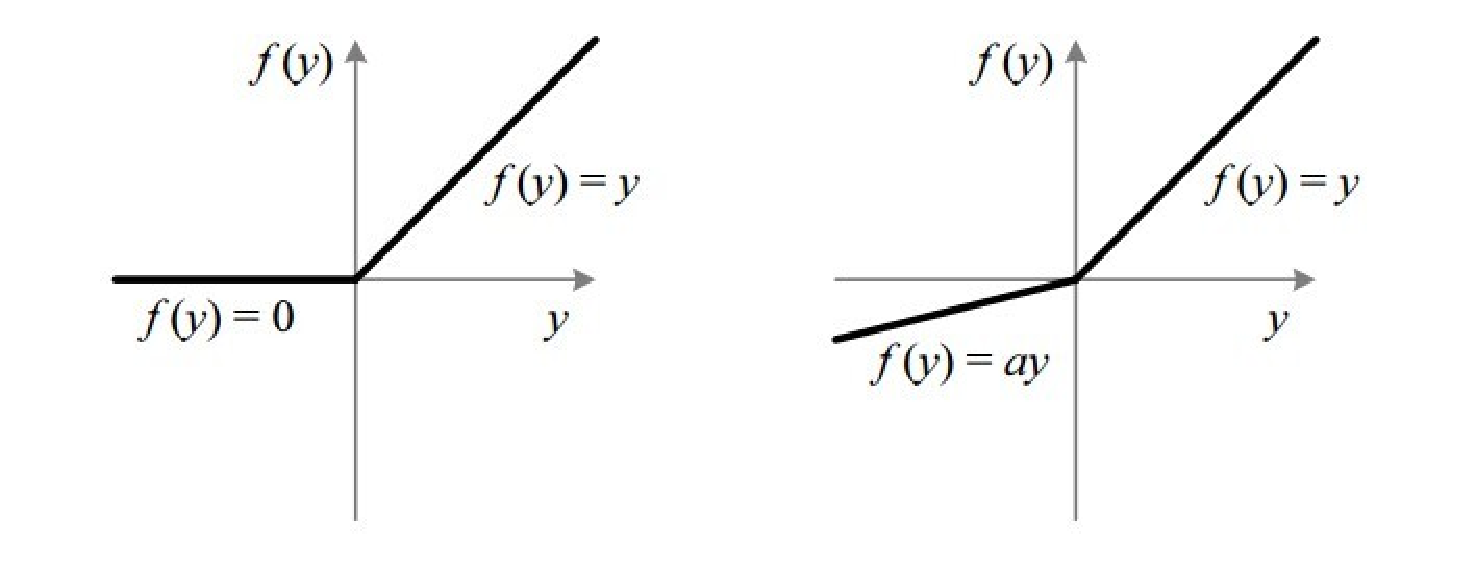
\includegraphics[width=1.0\linewidth]{Relu.pdf}
    	\caption{Comparision between ReLU (left) and Leaky ReLU (right)}
    	\label{fig:Relu}
    \end{figure}
	\footnote{https://towardsdatascience.com/activation-functions-neural-networks-1cbd9f8d91d6}
    
    
    
    \subsubsection{Dropout}
    Dropout is one of the newest but also most effective regularization techniques. It is a layer that accepts the dropout fraction as a parameter. It ranges from 0 to 1 and specifies the percentage of how many output features should be set to 0. \\
    Although at first glance, it may not be entirely clear how this contributes to the stability of the network, once you think about it it is actually conclusive. With this technique it is possible to break up conspiracies, as it is called by  the inventor Geoff Hinton\cite{JMLR:v15:srivastava14a}. In the end you want to force the network to form a robust representation of the input. This is done through introducing redundancy. By preventing the formation of insignificant patterns, overfitting can be tackled. By using dropout, especially at the end of the discriminator, we definitely could get better results over all.

    \subsection{Hyperparameters}

    We already discussed activation functions, specifically the usage of Leaky ReLU, already, nonetheless we want to point out an exception to that heuristic. Specifically, for original GANs it is accepted as standard to use a bounded activation function for the last layer of the Generator. Radford et al. \cite{radford2015unsupervised} argue that the model may "learn more quickly to saturate and cover space of the distribution" when going for a bounded activation function. We opted for tanh, sigmoid would be also a possible alternative. This rule, so to speak, is not true for extensions of the original GANs, like the Wasserstein GAN\cite{arjovsky2017wasserstein} which we cover later because it applies a linear activation function to its last layer of the Generator. Since GAN training is generally considered to be unstable, we tried to stick to prevalent conventions when choosing hyper parameters. \\
    We took Adam as optimizer which we preferred over RMSprop. We changed the learning rate in an interval from 0.0001 to 0.0004, with 0.0002 returning the best results. If the values are set too high, lets say 0.005, there was only a strong red or yellow tone recognizable on the pictures, without the possibility of interpreting other features. The Discriminator and the Generator both implemented the Adam optimizer with the same parameters, the same applies to the loss function, where we used binary crossentropy. \\
    With respect to the Discriminator, the choice definitely makes sense since binary crossentropy is designed for yes or no decisions. We cannot make judgements about the Generator however, first we would like to further adjust other hyperparameters and the network architecture before we experiment with the loss function.\\
    Finally, the samples we submitted to our testers were trained with between 9000 to 17000 epochs.

    \subsection{Evalution}

    There is no standard for Generative Adversarial Networks to evaluate the generated outcome. We therefore decided to use a mathematical evaluation method and the intuitive approach, namely by asking human inspectors for feedback. 

    \subsection{Inception Score}
    One wants to take two ideas into account when calculating the Inception Score. On one hand, that the individual image is highly meaningful (little entropy), on the other hand, that the images are as different as possible from one another. Two distributions are included for this evaluation. The label distribution returns a high value if the generated image could be clearly classified in a target category. The marginal distribution is optimally evenly distributed since all target classes should be served by the model if possible. Ultimately, these two distributions must be compared, for which the Kullback – Leibler divergence is used. If two unequal distributions are compared, a high value is calculated. The more dissimilar these distributions are, the higher the number will be, which is why a higher Inception Score is desirable. Let us consider the example of mode collapse in which the same image or a slight variation of it is produced regardless of the input. Since this is usually an image of higher quality, we receive a narrow label distribution. However, because there is little to no diversity among the generated images, the marginal distribution is also narrow. Due to the proximity of the two distributions, this leads to a low Inception Score. Finally we take the exponential of the result to increase the expressiveness of the number. We used the calculation of the score from this article. \footnote{https://machinelearningmastery.com/how-to-implement-the-inception-score-from-scratch-for-evaluating-generated-images/}Unfortunately, in most cases the Inception Score was not very meaningful for several reasons. The example of mode collapse at times occurred. In addition, our domain (burning houses, most of them wooden) is not directly represented in ImageNet database\footnote{http://www.image-net.org/}, from which the underlying Inception Classifier draws its classes, only boats houses or restaurants for example are available. Fire, the main feature of our dataset, is not present there either. Therefore, regardless of whether pictures were viewed by friends or by ourselves as of good quality, pictures received a low inception score or the same as pictures that we rated as of poor quality. We repeated this inspection process 10 times with 100 images per bad / good generator.

    \subsection{Judgement by Human Supervisor}

    Since the Inception Score did not turn out as applicable in this case, we primary had to rely on human judgement. On one hand, this makes sense, of course, since the image generated is ultimately intended for the human eye which can quickly discover any discrepancies to the real object or scene, given those differences are not too fine. Even if the accuracy of the checking of single images is more or less assured, the tester cannot check a large amount of samples, which is necessary for large networks with many output classes. As also mentioned by Ian Goodfellow in his book "Deep Learning" \cite{Goodfellow-et-al-2016}, humans are not able to find the lack of variation for a huge number of generated images. Luckily, our model is a less intricate one with only one output class. Whether the model has successfully learned the distribution is therefore a yes or no question. To get feedback, we kept putting pictures in a designated folder in google drive which we made accessible to the testers. We have set the test size to 100 pictures, because this gives more information about the average quality of the pictures. Nevertheless, it is still a reasonable size before the testers lose their motivation et cetera. The test subjects worked unpaid, which is why the task was performed by a group of friends of us. When presenting the pictures, however, we told half of the inspectors what they are expected to see in the pictures and for the other half we left room for interpretation. In the group without specifications, the answers were very wide-ranging, occasionally people tapped on fire due to the many shades of yellow and red. Houses or even burning houses could not be recognized. The instructed control group was able to detect the fire quite reliably, although the quality description still fluctuated greatly. In some of the pictures, outlines of houses could already be seen. Intuitively, of course it makes little sense to train the subjects to look for certain features. In the end, this should be done without outside help. Nevertheless, we were able to evaluate the quality of the individual features, in this case primarily fire, even if the overall picture of house plus fire plus environment is still quite vague. Overall, we are very satisfied with our testers. If we had used crowd-sourcing platforms, we would have had similar problems regarding motivation or concerning the set-up.

    \subsection{Prototype}
    We do not want to force everyone who wants to see the results of our project to download and run the code. We are of course happy about feedback, but we would also like to address people without a programming background. Therefore a prototype is available on our homepage \footnote{https://home.in.tum.de/~bindera/}. The model on that page was transformed from python to tensorflowjs using the provided tensorflowjs converter. We tried to keep the design and the code fairly clear. When you go to the page, you are only asked to enter the number of images to be generated. The required logic is completely written inside the index.html file. The styling takes place there as well.

